\documentclass[lettersize,journal]{IEEEtran}
\usepackage{booktabs}
\usepackage{colortbl}
\usepackage{supertabular}
\usepackage{flushend}
\usepackage{amsmath,amsfonts}
\usepackage{array}
\usepackage{textcomp}
\usepackage{tikz}
\usetikzlibrary{positioning}
\usetikzlibrary{math}
\usetikzlibrary{shapes}
\usepackage{pgfplots}
\usepackage{pgfplotstable}
\pgfplotsset{compat=1.7}
\usepgfplotslibrary{dateplot}
\setcounter{MaxMatrixCols}{20}
\usepackage{subfig}
\usepackage{stfloats}
\usepackage{url}
\usepackage{verbatim}
\usepackage{graphicx}
\usepackage{mathtools}
\usepackage{balance}

% import custom function definitions
\usepackage{ifthen}
\input{\rootdirectorytwo/functions/pgf_setup}
\makeatletter
\@ifundefined{makeComparisonBarChartFourPTwo}{%
\newcommand\makeComparisonBarChartFourPTwo[6]{%
	\pgfplotstableread[col sep=comma]{#1}\table
	\begin{tikzpicture}
		\begin{axis}[SmallBarPlot, xticklabels from table={\table}{type}, ylabel=#2]
			\addplot [fill=blue!20, bar width=0.1] table [x expr=\coordindex*0.6 + 0.3, y=#3]{\table};
			\addlegendentry{#3}
			\addplot [fill=green!20, bar width=0.1] table [x expr=\coordindex*0.6 + 0.3, y=#4]{\table};
			\addlegendentry{#4}
			\addplot [fill=red!20, bar width=0.1] table [x expr=\coordindex*0.6 + 0.3, y=#5]{\table};
			\addlegendentry{#5} 
			\addplot [fill=purple!20, bar width=0.1] table [x expr=\coordindex*0.6 + 0.3, y=#6]{\table};
			\addlegendentry{#6}
			\legend{#3, #4, #5, #6}
		\end{axis}
	\end{tikzpicture} 
}
}
\makeatother
 
\input{\rootdirectorytwo/functions/makeComparisonBarChartLogPTwo}
\makeatletter
\@ifundefined{makeComparisonPowerPTwo}{%
\newcommand\makeComparisonPowerPTwo[5]{%
	\pgfplotstableread[col sep=comma]{#1}\firstTable
	\pgfplotstableread[col sep=comma]{#2}\secondTable
	\centering
	\begin{tikzpicture}
		\begin{axis}[SmallTimeSeriesPlot, ymin=-1, ymax=750, xlabel=Time (hr:min), ylabel=#3, legend style={nodes={scale=0.7}}]
			\addplot[blue, smooth] table [x = {time}, y = {meanBusPower}]{\firstTable};
			\addplot[red, smooth] table [x = {time}, y = {meanBusPower}]{\secondTable};
			\addplot[brown, smooth] table [x = {time}, y = {loadPower}]{\firstTable};
			\filldraw[fill=gray!40, opacity=0.3](625,0) rectangle (917,750);
			\addlegendimage{line width=10pt, color=gray!40, draw opacity=0.5}
			\legend{#4, #5, Uncontrolled Load, On-Peak Time}
		\end{axis} 
	\end{tikzpicture} 
}
}
\makeatother

\input{\rootdirectorytwo/functions/makeComparisonTotalPowerPTwo}

 
\hyphenation{op-tical net-works semi-conduc-tor IEEE-Xplore}
\def\BibTeX{{\rm B\kern-.05em{\sc i\kern-.025em b}\kern-.08em
    T\kern-.1667em\lower.7ex\hbox{E}\kern-.125emX}} 
\usepackage[backend=bibtex, style=numeric, sorting=none]{biblatex}
\bibliography{references}
\begin{document}
\title{A Bin Packing Approach to Minimize Charging Cost for Electric Bus Fleets}
\author{Daniel Mortensen, Jacob Gunther, Greg Droge\thanks{}}

\markboth{Transactions on Intelligent Transportation Systems}%
{}

\maketitle 
\begin{abstract}
\end{abstract}
\begin{IEEEkeywords}
	Battery Electric Buses, Cost Minimization, Multi-Rate Charging, Mixed Integer Linear Program
\end{IEEEkeywords}





\section{Introduction}
\begin{enumerate}
	\item Electric buses are good because
		\begin{enumerate}
			\item They incur less maintenance \cite{poornesh_comparative_2020}(Poornesh et al.)
			\item They are eco-friendly \cite{kato_comparative_2013}
				\begin{enumerate}
					\item Provide access to renewable energy \cite{cheng_smart_2020}
					\item Give off zero emissions
				\end{enumerate}
		\end{enumerate}
	\item Electric buses struggle with
		\begin{enumerate}
			\item Extended charge times impact logistics (can take anyware from 100 minutes to 8 hours for a full charge)
			\item Extended charge times are reduced with high power chargers
			\item High charge rates taxe electrical infrastructure and increase the overall cost of energy. \cite{stahleder_impact_2019}, \cite{deb_impact_2017}, \cite{boonraksa_impact_2019}
		\end{enumerate}
	\item Managing electric bus fleet logistics can be handled on two levels
		\begin{enumerate}
			\item installation design: addresses questions such as what should the routes be, where should chargers be located, and what kinds of charging hardware do we use.
			\item charge scheduling: addresses the question of when should buses charge given the constraints from the installaion. 
		\end{enumerate}
	\item In most circumstances, hardare for charging is already installed or options are limited (with some exceptions (Ojer, et al)) and thus, the majority of work focuses on optimally utilizing a variety of charging hardware including
		\begin{enumerate}
			\item Dynamic overhead charging \cite{csonka_optimization_2021}
			\item Dynamic inductive charging \cite{jeong_automatic_2018} \cite{balde_electric_2019}
			\item battery swapping \cite{jain_battery_2020} \cite{xian_zhang_optimal_2016}
			\item stationary charging (A. Jahic),\cite{whitaker_network_nodate}
		\end{enumerate}
	\item each hardare type has its merits. Both the dynamic overhead and inductive charging eliminate the need for planning and down time as buses are charged while in service, but require expensive infrastructure that may not be feasible to install or purchase.
	\item battery swapping doesn't require any type of hardware installation and removes limitations imposed by route schedules, but requires specialized tools and/or automation.
	\item stationary charging is the least invasive form of bus charging because it only requires charging hardware at specific locations and makes no changes to bus batteries. 
	\item stationary charging is accomplished through forming intelligent charge plans. These plans can take on multiple considerations including bus availability, environmental impact \cite{zhou_bi-objective_2021}, battery health \cite{houbbadi_optimal_2019}, and the cost of electricity.
	\item electrical cost is based on the cost of generating power, and the cost of maintaining the distribution hardare. Large charge rates stress the existing infrastructure and therefore incur additional cost.
	\item Methods to decrease energy expenses have been formed by decreasing the load exigence \cite{cheng_smart_2020}, \cite{ojer_development_2020}, \cite{qin_numerical_2016}, \cite{bagherinezhad_spatio-temporal_2020} or minimising cost directly.
	\item Contributions: This work builds on \cite{brown_position_nodate} by encorporating the rate schedule from \cite{rocky_mountain_power_rocky_2021} as the linear objective function from \cite{mortensen_comprehensive_2020} which includes on-peak and off-peak rates, uncontrolled loads, and rate-sensative fees known as demand and facilities charges.  
	\item The rest of this paper is organized as follows: 
\end{enumerate}

\newpage temp \newpage
\section{Problem Formulation}
Solving the bus charge problem requires knowing when, and on which charger a bus must charge, indicating a solution with two dimensions.  The first dimension represents time continuously from left to right, and the second describes the buses as shown in Fig. \ref{fig:busTime1}.
\begin{figure*}
	\centering
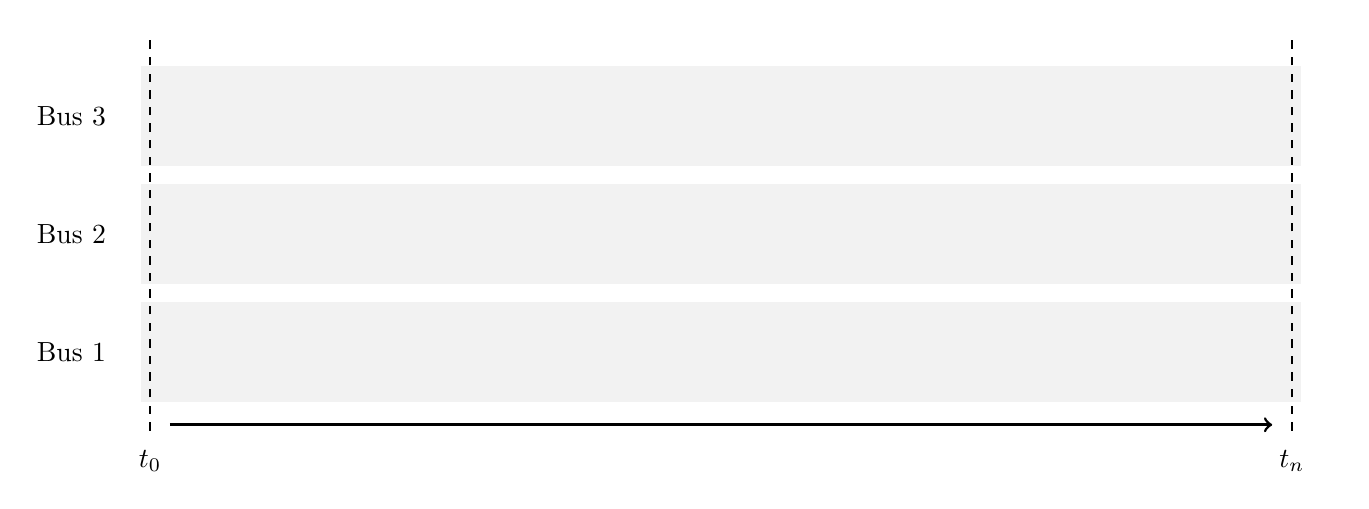
\begin{tikzpicture}
	\node[rectangle, fill=gray!10, minimum width=5.8in, minimum height=0.5in](bus1Box) at (7.75,1){};
	\node(bus1BoxLabel) at (-0.5, 1){Bus 1}; 

	\node[rectangle, fill=gray!10, minimum width=5.8in, minimum height=0.5in](bus2Box) at (7.75,2.5){};
	\node(bus1BoxLabel) at (-0.5, 2.5){Bus 2};

	\node[rectangle, fill=gray!10, minimum width=5.8in, minimum height=0.5in](bus3Box) at (7.75,4){};
	\node(bus1BoxLabel) at (-0.5, 4){Bus 3};

	\node[label=below:$t_0$](origin) at (0.5,0){};
	\node(yAxes) at (15.5,0){};
	\node(xAxes) at (0.5,5){};
	\node[label=below:$t_n$](bottomRight) at (15,0){};
	\node(topRight) at (15,5){};
	\draw[dashed, line width=0.5pt] (origin.center) -- (xAxes.center); 
	\draw[dashed, line width=0.5pt] (bottomRight.center) -- (topRight.center);
	\node(t0) at (0.75,-0.05){};
	\node(tn) at (14.75,-0.05){};
	\draw[->, line width=1pt] (t0.north) -- (tn.north); 
\end{tikzpicture}
	\caption{Description of the bus and time axis}
	\label{fig:busTime1}
\end{figure*}

\par Each bus follows a schedule and is in the station during predefined times. When a bus is in the station, it is available to charge.  Bus availability is described in terms of it's arrival and departure times, where the bus's $n^{\text{th}}$ stop begins at arrival time $n$, or $a_n$ and terminates at the $n^{\text{th}}$ departure time, $d_n$ (see Fig. \ref{fig:busTime2}). 
\begin{figure*}
\centering
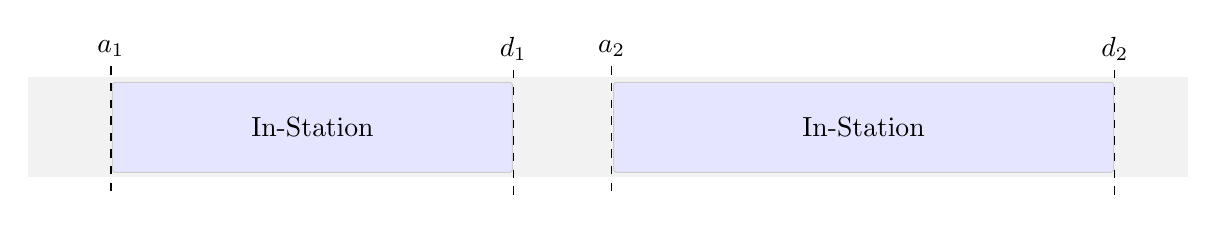
\begin{tikzpicture} 
	\node[rectangle, fill=gray!10, minimum width=5.8in, minimum height=0.5in](busAvail) at (7.75,4){}; 

	\node[rectangle, draw=blue!10!black!20, fill=blue!10, minimum width=2in, minimum height=0.45in, rounded corners=1pt](busAvail1) at (4,4){In-Station};
	\node[rectangle, draw=blue!10!black!20, fill=blue!10, minimum width=2.5in, minimum height=0.45in, rounded corners=1pt](busAvail2) at (11,4){In-Station};

	\node(firstATop) at (1.44,5){$a_1$};
	\node(firstABtm) at (1.44,3.1){};
	\draw[dashed, line width=0.5pt](firstATop) -- (firstABtm.center);
	\node(firstDTop) at (6.55,5){$d_1$};
	\node(firstDBtm) at (6.55,3.1){};
	\draw[dashed, line width=0.5pt](firstDTop) -- (firstDBtm.center);

	\node(secondATop) at (7.8,5){$a_2$};
	\node(secondABtm) at (7.8,3.1){};
	\draw[dashed, line width=0.5pt](secondATop) -- (secondABtm.center);
	\node(secondDTop) at (14.19,5){$d_2$};
	\node(secondDBtm) at (14.19,3.1){};
	\draw[dashed, line width=0.5pt](secondDTop) -- (secondDBtm.center);


\end{tikzpicture}
\caption{Bus availability}
\label{fig:busTime2}
\end{figure*}

\par A bus can be assigned to charge for a time interval where the bus is in the station. The charge start time during the $n^{\text{th}}$ stop is denoted $c_n$ and the stop-charge time is denoted $s_n$ as shown in Fig. \ref{fig:busTime3}. 
\begin{figure*}
\centering
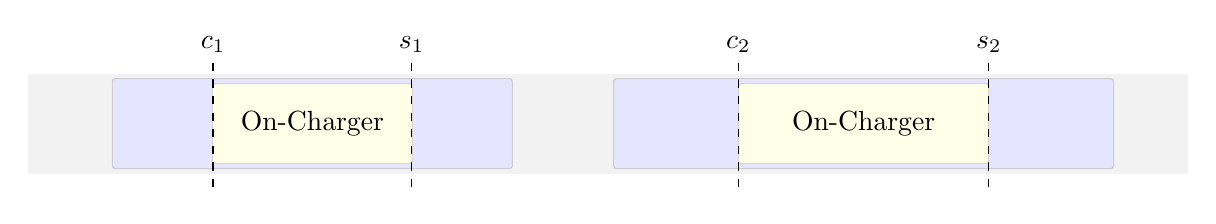
\begin{tikzpicture} 
	\node[rectangle, fill=gray!10, minimum width=5.8in, minimum height=0.5in](busSched) at (7.75,1){}; 

	\node[rectangle, draw=blue!10!black!20, fill=blue!10, minimum width=2in, minimum height=0.45in, rounded corners=1pt](busAvail1) at (4,1){In-Station};
	\node[rectangle, draw=blue!10!black!20, fill=blue!10, minimum width=2.5in, minimum height=0.45in, rounded corners=1pt](busAvail2) at (11,1){In-Station};

	\node[rectangle, draw=yellow!10!black!20, fill=yellow!10, minimum width=1in, minimum height=0.4in, rounded corners=1pt](busAvail1) at (4,1){On-Charger};
	\node[rectangle, draw=yellow!10!black!20, fill=yellow!10, minimum width=1.25in, minimum height=0.4in, rounded corners=1pt](busAvail2) at (11,1){On-Charger};


	\node(firstATop) at (2.74,2){$c_1$};
	\node(firstABtm) at (2.74,0.2){};
	\draw[dashed, line width=0.5pt](firstATop) -- (firstABtm.center);
	\node(firstDTop) at (5.26,2){$s_1$};
	\node(firstDBtm) at (5.26,0.2){};
	\draw[dashed, line width=0.5pt](firstDTop) -- (firstDBtm.center);

	\node(secondATop) at (9.41,2){$c_2$};
	\node(secondABtm) at (9.41,0.2){};
	\draw[dashed, line width=0.5pt](secondATop) -- (secondABtm.center);
	\node(secondDTop) at (12.59,2){$s_2$};
	\node(secondDBtm) at (12.59,0.2){};
	\draw[dashed, line width=0.5pt](secondDTop) -- (secondDBtm.center);


\end{tikzpicture}
\caption{Bus Charging}
\label{fig:busTime3}
\end{figure*}

The relationship between the arrival, departure, and charge intervals for the $i^{\text{th}}$ bus at the $j^{\text{th}}$ stop can be expressed as a set of inequality constraints such that
\begin{align}
	a_{ij} &< c_{ij} \\
	c_{ij} &< s_{ij} \\
	s_{ij} &< d_{ij}
\end{align}
Which can be expressed in standard form as
\begin{align}
	-c_{ij} &< -a_{ij}\\
	c_{ij} - s_{ij} &< 0\\
	s_{ij} &< d_{ij}
\end{align}
and finally, 
\begin{align}\label{eqn:timeConstraint}
	\begin{bmatrix} -1 & 0 \\
	                 1 & -1 \\
		0 & 1\end{bmatrix} \begin{bmatrix} c_{ij} \\ s_{ij}\end{bmatrix} \le \begin{bmatrix}-a_{ij} \\ 0 \\ d_{ij} \end{bmatrix}.
\end{align}

\par A charge plan can be formulated by reserving time slots at chargers when buses need to charge (see Fig. \ref{fig:busTime4}).
\begin{figure*}
	\centering
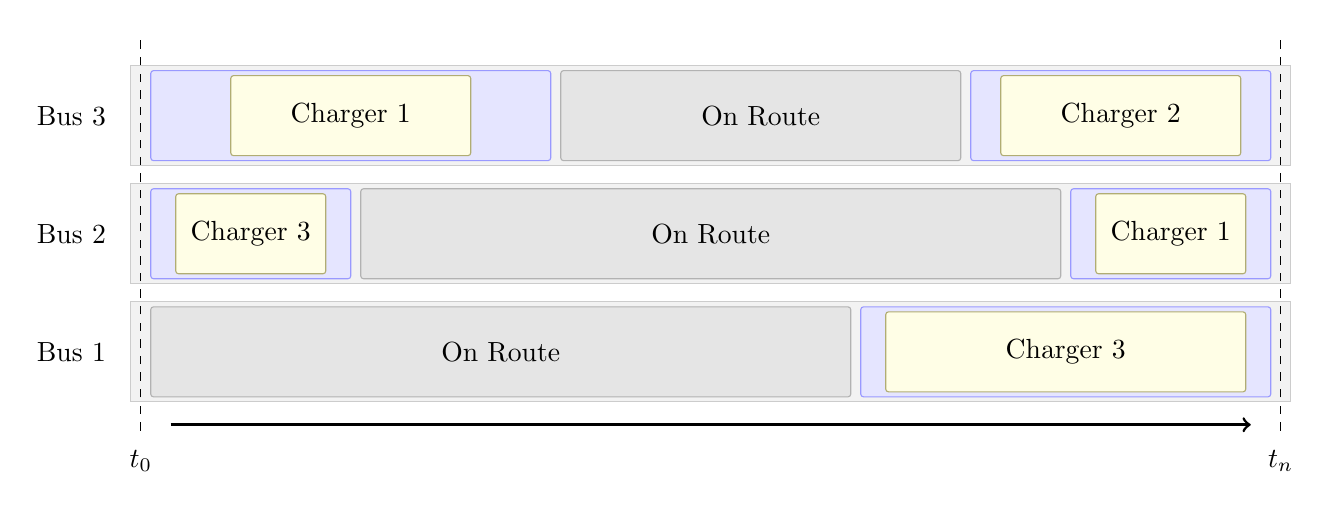
\begin{tikzpicture}
	\node[rectangle, draw=gray!40, fill=gray!10, minimum width=5.8in, minimum height=0.5in](charger1Box) at (3in,1){};
	\node(bus1BoxLabel) at (-0.5, 1){Bus 1}; 

	\node[rectangle, draw=gray!40, fill=gray!10, minimum width=5.8in, minimum height=0.5in](charger2Box) at (3in,2.5){};
	\node(bus1BoxLabel) at (-0.5, 2.5){Bus 2};

	\node[rectangle, draw=gray!40, fill=gray!10, minimum width=5.8in, minimum height=0.5in](charger3Box) at (3in,4){};
	\node(bus1BoxLabel) at (-0.5, 4){Bus 3};

	\node[label=below:$t_0$](origin) at (0.15in,0){};
	\node(xAxes) at (0.15in,5){};
	\node[label=below:$t_n$](bottomRight) at (5.85in,0){};
	\node(topRight) at (5.85in,5){};
	\draw[dashed, line width=0.5pt] (origin.center) -- (xAxes.center); 
	\draw[dashed, line width=0.5pt] (bottomRight.center) -- (topRight.center);
	\node(t0) at (0.3in,-0.05){};
	\node(tn) at (5.7in,-0.05){};
	\draw[->, line width=1pt] (t0.north) -- (tn.north); 

	% draw bus 3 boxes
	\node[rectangle, draw=blue!40, fill=blue!10, minimum width=2in, minimum height=0.45in, rounded corners=1pt](bus1Avail1) at (1.2in,4){};
	\node[rectangle, draw=yellow!50!black!70, fill=yellow!10, minimum width=1.2in, minimum height=0.4in, rounded corners=1pt](bus1Time1) at (1.2in,4){Charger 1};

	\node[rectangle, draw=black!30, fill=black!10, minimum width=2in, minimum height=0.45in, rounded corners=1pt](bus2Time1) at (3.25in,4){On Route};

	\node[rectangle, draw=blue!40, fill=blue!10, minimum width=1.5in, minimum height=0.45in, rounded corners=1pt](bus1Avail1) at (5.05in,4){};
	\node[rectangle, draw=yellow!50!black!70, fill=yellow!10, minimum width=1.2in, minimum height=0.40in, rounded corners=1pt](bus3Time1) at (5.05in,4){Charger 2};

	% draw bus 2 boxes
	\node[rectangle, draw=blue!40, fill=blue!10, minimum width=1in, minimum height=0.45in, rounded corners=1pt](bus1Avail1) at (0.7in,2.5){};
	\node[rectangle, draw=yellow!50!black!70, fill=yellow!10, minimum width=0.75in, minimum height=0.4in, rounded corners=1pt](free1) at (0.7in,2.5){Charger 3};

	\node[rectangle, draw=black!30, fill=black!10, minimum width=3.5in, minimum height=0.45in, rounded corners=1pt](bus3Time2) at (3.0in,2.5){On Route};

	\node[rectangle, draw=blue!40, fill=blue!10, minimum width=1.0in, minimum height=0.45in, rounded corners=1pt](bus1Avail1) at (5.3in,2.5){};
	\node[rectangle, draw=yellow!50!black!70, fill=yellow!10, minimum width=0.75in, minimum height=0.4in, rounded corners=1pt](free2) at (5.3in,2.5){Charger 1};

	% draw bus 1 boxes 
	\node[rectangle, draw=black!30!, fill=black!10, minimum width=3.5in, minimum height=0.45in, rounded corners=1pt](bus3Time2) at (1.95in,1){On Route}; 

	\node[rectangle, draw=blue!40, fill=blue!10, minimum width=2.05in, minimum height=0.45in, rounded corners=1pt](bus1Avail1) at (4.775in,1){};
	\node[rectangle, draw=yellow!50!black!70, fill=yellow!10, minimum width=1.8in, minimum height=0.4in, rounded corners=1pt](bus1Time2) at (4.775in,1){Charger 3};
\end{tikzpicture}
	\caption{Reserving time slots on chargers}
	\label{fig:busTime4}
\end{figure*}

	Note how there are several decisions that go into the charge schedule, which is made up to which bus charges at which charger at which time. 
	\par The variables for time have already been discussed in equation \ref{eqn:timeConstraint}, but variables for which charger have not been given.  Let $\sigma_{ijk}$ be a binary variable that is $1$ when bus $i$ charges during the $j^{\text{th}}$ stop at charger $k$. Because a bus can only charge at one charger at a time, we also constraint $\sigma$ such that
	\begin{equation}
		\begin{aligned}
			\sum_k \sigma_{ijk} \le 1 \ \forall i,j
		\end{aligned}
	\end{equation}
	$\sigma_{ijk}$ is necessary to eliminate situations where more then one bus is assigned to a charger at the same time. Note that this can only happen when $a_{ij}$ for bus $j$ is less than $d_{i^{'}j^{'}}$ for bus $j^{'}$ as shown in Fig. \ref{fig:potentialOverlap}. Charging overlap can be avoided by constraining
	\begin{figure}
	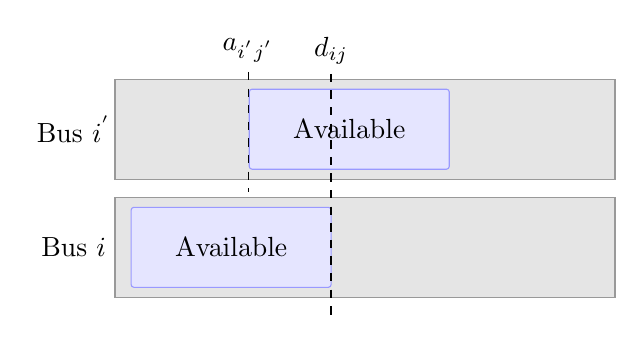
\begin{tikzpicture} 
		\node[rectangle, draw=black!40, fill=black!10, minimum width=2.5in, minimum height=0.5in](charger1Box) at (3.2,1){};
		\node(bus1BoxLabel) at (-0.5, 1){Bus $i$}; 
		\node[rectangle, draw=black!40, fill=black!10, minimum width=2.5in, minimum height=0.5in](charger2Box) at (3.2,2.5){};
		\node(bus1BoxLabel) at (-0.5, 2.5){Bus $i^{'}$};
		\node[rectangle, draw=blue!40, fill=blue!10, minimum width=1in, minimum height=0.4in, rounded corners=1pt] at (1.5,1){Available};
		\node[rectangle, draw=blue!40, fill=blue!10, minimum width=1in, minimum height=0.4in, rounded corners=1pt] at (3,2.5){Available};
		\node(aJPrimeHigh) at (1.72,3.5){$a_{i^{'}j^{'}}$};
		\node(aJPrimeLow) at (1.72,1.7){};
		\node(dJHigh) at (2.77,3.5){$d_{ij}$};
		\node(dJLow) at (2.77,0.0){};
		\draw[dashed, line width=0.5pt] (aJPrimeHigh) -- (aJPrimeLow.center);
		\draw[dashed, line width=0.5pt] (dJHigh) -- (dJLow);
	\end{tikzpicture}
	\caption{Potential Overlap}
	\label{fig:potentialOverlap}
\end{figure}


	
	\begin{align}\label{eqn:overlapConstraints1}
	c_{i^{'}j^{'}} > s_{ij}.
\end{align}
However, this constraint is only necessary when both bus stops are designated for charging. This can be remedied as
	\begin{align}\label{eqn:overlapConstraints2}
		c_{i^{'}j^{'}} - s_{ij} > M\left[(\sigma_{i^{'}j^{'}k^{'}} + \sigma_{ijk}) - 2\right]
	\end{align}
	Where $M = 2\cdot\text{nTime}$. When $(\sigma_{i^{'}j^{'}k^{'}} + \sigma_{ijk}) < 2$, then equation \ref{eqn:overlapConstraints2} is trivially satisfied for all values of $c_{i^{'}j^{'}}$ and $s_{ij}$ and when $\sigma_{i^{'}j^{'}k^{'}} = \sigma_{ijk} = 1$, equation \ref{eqn:overlapConstraints2} simplifies to equation \ref{eqn:overlapConstraints1}. Equation \ref{eqn:overlapConstraints1} can be expressed in standard form as 
	\begin{align}\label{eqn:overlapConstraints3}
		c_{i^{'}j^{'}} - s_{ij} - M\sigma_{i^{'}j^{'}k^{'}} - M\sigma_{ijk} &\ge -2M \\
		-c_{i^{'}j^{'}} + s_{ij} + M\sigma_{i^{'}j^{'}k^{'}} + M\sigma_{ijk} &\le 2M \\
		\begin{bmatrix} -1 & 1 & M & M\end{bmatrix} \begin{bmatrix}c_{i^{'}j^{'}}\\ s_{ij} \\ \sigma_{i^{'}j^{'}k^{'}}\\ \sigma{ijk} \end{bmatrix} &\le 2M
	\end{align}
	The constraints in equation \ref{eqn:overlapConstraints3} can be repeated for all instances where overlap is possible and concatenated into a single matrix such that
	\begin{equation}
		A\mathbf{y} \le \mathbf{1}\cdot 2M
	\end{equation}




\section{Battery State of Charge}
TODO:
\begin{itemize}
	\item find variable for power and substitute
	\item make arrows for delta give space between arrow tip and box
	\item begin more thorough pass through on text and explaining where things go
\end{itemize}
BEBs must also maintain their state of charge above a minimum threshold. Let $h_{ij+1}$ be the state of charge for bus $i$ at the beginning of stop $j$. Each bus has an initial state of charge defined by $h_{i0}$ as shown in figure \ref{fig:hPlacement}. 
\begin{figure*}
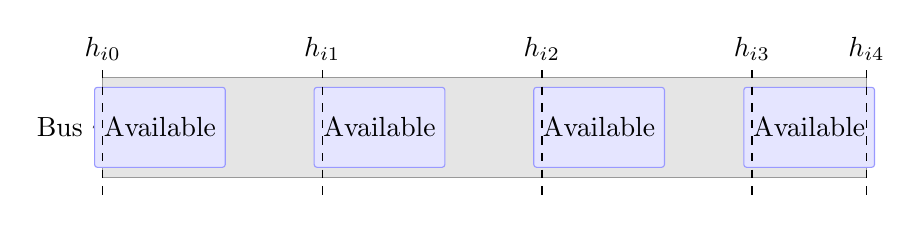
\begin{tikzpicture}
\node[rectangle, draw=black!40, fill=black!10, minimum width=0.8\textwidth, minimum height=0.5in](charger1Box) at (0.5\textwidth,1){};
	\node(bus1BoxLabel) at (0.065\textwidth, 1){Bus $i$}; 
	\node[rectangle, draw=blue!40, fill=blue!10, minimum width=0.12\textwidth, minimum height=0.4in, rounded corners=1pt] at (0.16\textwidth,1){Available};
	\node[rectangle, draw=blue!40, fill=blue!10, minimum width=0.12\textwidth, minimum height=0.4in, rounded corners=1pt] at (0.39\textwidth,1){Available};
	\node[rectangle, draw=blue!40, fill=blue!10, minimum width=0.12\textwidth, minimum height=0.4in, rounded corners=1pt] at (0.62\textwidth,1){Available};
	\node[rectangle, draw=blue!40, fill=blue!10, minimum width=0.12\textwidth, minimum height=0.4in, rounded corners=1pt] at (0.84\textwidth,1){Available};

	\node(h0High) at (0.1\textwidth,2){$h_{i0}$};
	\node(h0Low) at (0.1\textwidth,0.05){};
	\draw[dashed, line width=0.5pt] (h0High) -- (h0Low.center);

	\node(h1High) at (0.33\textwidth,2){$h_{i1}$};
	\node(h1Low) at (0.33\textwidth,0.05){};
	\draw[dashed, line width=0.5pt] (h1High) -- (h1Low.center);

	\node(h0High) at (0.56\textwidth,2){$h_{i2}$};
	\node(h0Low) at (0.56\textwidth,0.05){};
	\draw[dashed, line width=0.5pt] (h0High) -- (h0Low.center);

	\node(h0High) at (0.78\textwidth,2){$h_{i3}$};
	\node(h0Low) at (0.78\textwidth,0.05){};
	\draw[dashed, line width=0.5pt] (h0High) -- (h0Low.center);

	\node(h0High) at (0.9\textwidth,2){$h_{i4}$};
	\node(h0Low) at (0.9\textwidth,0.05){};
	\draw[dashed, line width=0.5pt] (h0High) -- (h0Low.center);
\end{tikzpicture}
\caption{State of Charge Variables}
\label{fig:hPlacement}
\end{figure*}

This can be constrained as
\begin{equation}
	d_{i0} = \text{initialSoc}_{i} \ \forall i.
\end{equation}
\begin{figure*}
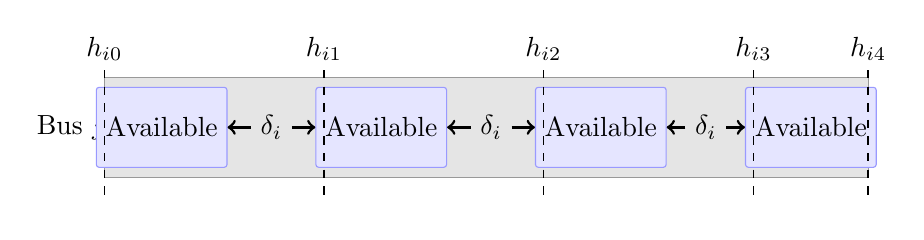
\begin{tikzpicture}
\node[rectangle, draw=black!40, fill=black!10, minimum width=0.8\textwidth, minimum height=0.5in](charger1Box) at (0.5\textwidth,1){};
	\node(bus1BoxLabel) at (0.065\textwidth, 1){Bus $j$}; 
	\node[rectangle, draw=blue!40, fill=blue!10, minimum width=0.12\textwidth, minimum height=0.4in, rounded corners=1pt](avail1) at (0.16\textwidth,1){Available};
	\node[rectangle, draw=blue!40, fill=blue!10, minimum width=0.12\textwidth, minimum height=0.4in, rounded corners=1pt](avail2) at (0.39\textwidth,1){Available};
	\node[rectangle, draw=blue!40, fill=blue!10, minimum width=0.12\textwidth, minimum height=0.4in, rounded corners=1pt](avail3) at (0.62\textwidth,1){Available};
	\node[rectangle, draw=blue!40, fill=blue!10, minimum width=0.12\textwidth, minimum height=0.4in, rounded corners=1pt](avail4) at (0.84\textwidth,1){Available};

	\node(h0High) at (0.1\textwidth,2){$h_{i0}$};
	\node(h0Low) at (0.1\textwidth,0.05){};
	\draw[dashed, line width=0.5pt] (h0High) -- (h0Low.center);

	\node(h1High) at (0.33\textwidth,2){$h_{i1}$};
	\node(h1Low) at (0.33\textwidth,0.05){};
	\draw[dashed, line width=0.5pt] (h1High) -- (h1Low.center);

	\node(h0High) at (0.56\textwidth,2){$h_{i2}$};
	\node(h0Low) at (0.56\textwidth,0.05){};
	\draw[dashed, line width=0.5pt] (h0High) -- (h0Low.center);

	\node(h0High) at (0.78\textwidth,2){$h_{i3}$};
	\node(h0Low) at (0.78\textwidth,0.05){};
	\draw[dashed, line width=0.5pt] (h0High) -- (h0Low.center);

	\node(h0High) at (0.9\textwidth,2){$h_{i4}$};
	\node(h0Low) at (0.9\textwidth,0.05){};
	\draw[dashed, line width=0.5pt] (h0High) -- (h0Low.center);

	\node(delta1) at (0.275\textwidth,1){$\delta_i$};
	\draw[->, line width=1pt] (delta1.west) -- (avail1.east);
	\draw[->, line width=1pt] (delta1.east) -- (avail2.west);
	\node(delta2) at (0.505\textwidth,1){$\delta_i$}; 
	\draw[->, line width=1pt] (delta2.west) -- (avail2.east);
	\draw[->, line width=1pt] (delta2.east) -- (avail3.west);
	\node(delta3) at (0.73\textwidth,1){$\delta_i$}; 
	\draw[->, line width=1pt] (delta3.west) -- (avail3.east);
	\draw[->, line width=1pt] (delta3.east) -- (avail4.west);
\end{tikzpicture}
\caption{Placement for $\delta_i$}
\label{fig:hPlacement}
\end{figure*}

The transition from one start to the next is computed as
\begin{equation}
	h_{ij} = h_{ij-1} - \delta_i + \left(\sum_k\sigma_{ijk}\right )\text{power}\cdot(d_{ij} - a_{ij}) 
\end{equation}
but because this introduces a bilinear term, we can alternatively express this constraint as
\begin{equation} \begin{aligned}
	h_{ij} & \le h_{ij-1} - \delta_i + \text{power}\cdot(d_{ij} - a_{ij}) - M(1 - \sum_k\sigma_{ijk})\\
	h_{ij} & \ge h_{ij-1} - \delta_i + \text{power}\cdot(d_{ij} - a_{ij}) + M(1 - \sum_k\sigma_{ijk})\\
	h_{ij} & \le h_{ij-1} - \delta_i - M\sum_k\sigma_{ijk}\\
	h_{ij} & \ge h_{ij-1} - \delta_i + M\sum_k\sigma_{ijk}\\
\end{aligned} \end{equation}
Which can be expressed in standard form as
\begin{equation} \begin{aligned}
	h_{ij} - h_{ij-1} - \text{power}\cdot d_{ij} + \text{power}\cdot a_{ij} - M\sum_k\sigma_{ijk} &\le -\left(\delta_i + M\right) \\
	-h_{ij} + h_{ij-1} + \text{power}\cdot d_{ij} - \text{power}\cdot a_{ij} - M\sum_k\sigma_{ijk} &\le \delta_i - M \\
	h_{ij} - h_{ij-1} + M\sum_k\sigma_{ijk} &\le -\delta_i \\
	-h_{ij} + h_{ij-1} + M\sum_k\sigma_{ijk} & \le \delta_i \\
\end{aligned} \end{equation}
and finally,
\begin{equation} \begin{aligned}
	\begin{bmatrix}1  & -1 & -\text{power} & \text{power}   & -M_k \\
		       -1 & 1  & \text{power}  & -\text{power}  & -M_k \\
		       1  & -1 & 0             & 0              & M_k  \\
		       -1 & 1  & 0             & 0              & M_k  \\
	\end{bmatrix}
	\begin{bmatrix}h_{ij} \\ h_{ij-1} \\ d_{ij} \\ a_{ij} \\ \sigma_{ijk} \end{bmatrix} \le 
		\begin{bmatrix}-\delta_i - M \\ \delta_i - M \\ -\delta_i \\ \delta_i \end{bmatrix}
\end{aligned} \end{equation}
If the bus end the day in the station (as is common), there is one final state of charge value that is computed as above without a route discharge parameter as
\begin{equation}
\begin{bmatrix}1  & -1 & -\text{power} & \text{power}   & -M_k \\
		       -1 & 1  & \text{power}  & -\text{power}  & -M_k \\
		       1  & -1 & 0             & 0              & M_k  \\
		       -1 & 1  & 0             & 0              & M_k  \\
	\end{bmatrix}
	\begin{bmatrix}h_{ij} \\ h_{ij-1} \\ d_{ij} \\ a_{ij} \\ \sigma_{ijk} \end{bmatrix} \le 
		\begin{bmatrix}- M \\ - M \\ 0 \\ 0 \end{bmatrix}.
\end{equation}
Now that the state of charge is defined, the final constraint ensures that the minimum battery state of charge is kept above some minimum threshold, denoted $h_{\text{min}}$. These constraints are given as
\begin{equation}
	-h_{ij} \le -h_{\text{min}} \ \forall i,j
\end{equation}
or 
\begin{equation} \begin{aligned}
	\begin{bmatrix}0 & \hdots & 0 & 1_{h} & 0 & \hdots & 0\end{bmatrix} \mathbf{y} &\le \mathbf{1}\cdot h_{\text{min}}\\ 
		H\mathbf{y} &\le \mathbf{b}_h
\end{aligned} \end{equation}


\section{Integrating Uncontrolled Loads}
Next, we desire to integrate the charge decisions with uncontrolled loads.  These loads are sampled discretly and so the results for the power use must be converted into a compatible format.  To start, define
\begin{align}
	k_0\cdot\Delta T + r_0&= c_{ijk} \\
	k_1\cdot\Delta T + r_1&= s_{ijk} \\
	k_1, k_0 \in \mathbb{Z} \\
	0 < r_0, r_1 < &\Delta T.
\end{align}
We desire to find binary vectors $\mathbf{s}_0$, $\mathbf{s}$, and $\mathbf{s_1}$ which act as selectors for times where a bus is on-ramping, charging, and off-ramping respectively. The on-ramping charging, and off-ramping periods will be used to represent power use from $k_0$ to $k_0 + 1$, $k_0 + 1$ to $k_1$ and $k_1$ to $k_1 + 1$ respectively. 
\par Let $\mathbf{i}$ be a vector of one-based integer indices such that $\mathbf{i}_w = w \ \forall w \in (1,\text{nTime})$. The values in $\mathbf{s}_0$ can be defined by the constraint
\begin{align}
	k_0 &= \mathbf{s}_0^T\mathbf{i} \\
	1 &= \mathbf{1}^T\mathbf{s}_0 \\
	\mathbf{s}_0 &\in \{0,1\}.
\end{align}
Similarly, the values for $\mathbf{s_1}$ can be defined as
\begin{align}
	k_1 &= \mathbf{s}_1^T\mathbf{i}\\
	1 &= \mathbf{1}^T\mathbf{s}_1 \\
	\mathbf{s}_1 &\in \{0,1\}.
\end{align}
The final piece is to define $\mathbf{s}$. The set of constraints can be described as follows: 
\begin{align}
	\mathbf{1}^T\mathbf{s} &= k_1 - k_0 - 1 \\
	\mathbf{s}_i\mathbf{i}_i &\le k_1 + M(1 - \mathbf{s}_i)\\
	\mathbf{s}_i\mathbf{i}_i &\ge k_0 - M(1 - \mathbf{s}_i)\\ 
\end{align}
where $M$ is $2\cdot\text{nTime}$.
\par We next define the average per use for each charger during an interval. The on-ramp intervals can be constrained as
\begin{align}
	p_{\text{on-ramp}} &= \frac{\text{powerRate}\cdot (\Delta T - r_0)}{\Delta T}\\
	p_{\text{off-ramp}} &= \frac{\text{powerRate}\cdot r_1}{\Delta T}\\
	p &= \text{powerRate},
\end{align}
where $p_0$, $p_1$, and $p$ represent the average power rate for the on-ramping, off-ramping, and charging intervals respectively.
The total average power use is calculated as 
\begin{align}\label{eqn:totalPower}
	\mathbf{p}_{\text{total}} = \mathbf{p} + \mathbf{s}_0\cdot p_0 + \mathbf{s}\cdot p + \mathbf{s}_1\cdot p_1
\end{align}
where $\mathbf{p}$ is the average power of the uncontrolled loads.
\par Note, however that the results from equation \ref{eqn:totalPower} contain a bilinear form. The first bilnear expression in  equation \ref{eqn:totalPower} can be rewritten as 
\begin{equation}
	\begin{aligned}
		p_0^w &\ge p_{\text{on-ramp}} - M(1 - s_0^w) \\
		p_0^w &\le p_{\text{on-ramp}} + M(1 - s_0^w) \\
		p_0^w &\ge -Ms_0^w \\
		p_0^w &\le Ms_0^w
	\end{aligned}
\end{equation}
and similarly the second as, 
\begin{equation}
	\begin{aligned}
		p_1^w &\ge p_{\text{off-ramp}} - M(1 - s_1^w) \\
		p_1^w &\le p_{\text{off-ramp}} + M(1 - s_1^w) \\
		p_1^w &\ge -Ms_1^w \\
		p_1^w &\le Ms_1^w.
	\end{aligned}
\end{equation}
An expression for the total power used can then be derived as
\begin{equation}
	\begin{aligned}
		\mathbf{p}_{\text{total}} = \mathbf{p} + \mathbf{p}_0 + \mathbf{p}_1 + \mathbf{s}\cdot p
	\end{aligned}
\end{equation}
TODO: 
\begin{enumerate}
	\item Figure out notation for each bus and how to integrate it into this framework
	\item flush out constraints and get into matrix/standard form
\end{enumerate}

\section{Objective Function\label{sec:objective}}
This work adopts the objective function developed in \textcolor{red}{insert reference to our prior paper here}, which implements the rate schedule from \textcolor{red}{insert reference to rocky mountain power}. The rate schedule in \textcolor{red}{insert reference to rocky mountain power rate schedule} is based off of two primary components: power, and energy.  
\par Power is billed per kW for the highest 15 minute average power over a desired period of time. It is common practice for power providers to designate "on-peak" periods when power is generally in high demand, and "off-peak" hours for all other time periods. 
\par The rate schedule given in \textcolor{red}{insert reference to rocky mountain here} assesses a fee for a users maximum average power during on-peak hours called the demand charge, and a user's overall maximum average power, called a facilities charge as shown in figure \ref{fig:charges}. 
\par Energy fees are also assessed per kWh of energy consumed with a higher rate for energy consumed during on-peak hours and a lower rate for energy consumed during off-peak hours.
\begin{figure*}
	\centering
	\begin{tabular}{c | c c c}
		            & On-Peak               & Off-Peak               & Both \\ \hline
		Energy      & On-Peak Energy Charge & Off-Peak Energy Charge & None \\
		Energy Rate & $u_{\text{e-on}}$     & $u_{\text{e-off}}$     & None \\
		Power       & Demand Charge         & None                   & Facilities Charge \\
		Power Rate  & $u_{\text{p-on}}$     & None                   & $u_{\text{p-all}}$
	\end{tabular}
	\caption{Description of the assumed billing structure}
	\label{fig:charges}
\end{figure*}

\subsection{Power Charges}
It is necessary to compute the maximum power both overall and for on-peak periods. In section \ref{sec:uncontrolled}, $\Delta T$ was used to denote the time offset between power samples and that each power reading would reflect the average power used in the previous interval. 
\par In this section, $\Delta T$ is set to 15 minutes, making $\mathbf{p}_{\text{total}}$ an expression of the 15 minute average power. Next, let $\mathcal{S}_{\text{on}}$ be the set of all indices belonging to on-peak time periods such that $j\in \mathcal{S}_{\text{on}} \Rightarrow p_j^{\text{total}} $ represents a 15 minute average during an on-peak interval.  Additionally, let $q_{\text{on}}$ be the maximum on-peak average power.  The constriants for determining the maximum on-peak average are defined as
\begin{equation} \begin{aligned}
	p_j^{\text{total}} &\le q_{\text{on}} \ \forall j \in \mathcal{S}_{\text{on}} \\
	p_j^{\text{total}} - q_{\text{on}} &\le 0 \ \forall j \in \mathcal{S}_{\text{on}}\\
	\begin{bmatrix}0 & \hdots & 0 & 1_j & 0 & \hdots & 0 & -1_{\text{on}} & 0 \end{bmatrix}\mathbf{y} &\le 0 \forall j\in \mathcal{S}_{on} \\
		A_{\text{ineq9}} &\le \mathbf{0}.
\end{aligned} \end{equation}
Because an increased value in $q_{\text{on}}$ is directly related to an increase in cost, the optimizer will minimize $q_{\text{on}}$ until it is equal to the maximum value in $\{p_j^{\text{total}} \ \forall j \in \mathcal{S}_{\text{on}}\}$. A similar proceedure can be used to derive a set of constraints for the overall maximum average power, denoted $q_{\text{all}}$, and is represented as
\begin{equation} 
	A_{\text{ineq10}}\mathbf{y} \le  \mathbf{0}.
\end{equation}
The charges for power are then expressed as 
\begin{equation} \begin{aligned}
	\text{power cost} &= q_{\text{on}}\cdot u_{\text{p-on}} + q_{\text{all}} \cdot u_{\text{p-all}} \\
	                  &= \begin{bmatrix}u_{\text{p-on}} & 0 & \hdots & 0 & u_{\text{p-all}} \end{bmatrix}\mathbf{y} \\
		          &= \mathbf{u}_{\text{p}}^T\mathbf{y}
\end{aligned}\end{equation}
where $u_{\text{p-on}}$ is the rate per kW for on-peak power use, or the demand charge and $u_{\text{p-all}}$ is the rate per kW for the overall maximum 15 minute average.
\subsection{Energy Charges}
Energy is defined as the integral of power over a length of time.  Because the values for power given in this work reflect an average power, the energy over a given period can be computed by multiplying the average power by the change in time, or $\Delta T$ such that
\begin{equation}\begin{aligned}
	\text{Total Energy} = \mathbf{1}^T\mathbf{p}_{\text{total}}\cdot \Delta T.
\end{aligned}\end{equation}
However, because the energy is billed for on-peak and off-peak time periods, we define two binary vectors $\mathbf{1}_{\text{on}}$ and $\mathbf{1}_{\text{off}}$ such that $1^{\text{on}}_j = 1$ when $p_j^{\text{total}}$ represents an average power from an on-peak time period and $1_{\text{off}} = 1$ when $p_j^{\text{total}}$ represents the average power usage for an off-peak interval. The on-peak and off-peak energy can be computed as
\begin{equation}\begin{aligned}
	\text{On-Peak Energy} = \mathbf{1}_{\text{on}}^T\mathbf{p}_{\text{total}}\cdot\Delta T\\
	\text{Off-Peak Energy} = \mathbf{1}_{\text{off}}^T\mathbf{p}_{\text{total}}\cdot\Delta T.
\end{aligned}\end{equation}
Let $u_{\text{e-on}}$ and $u_{\text{e-off}}$ represent the on-peak and off-peak energy rates respectively. The total cost for energy is computed as
\begin{equation} \begin{aligned}
	\text{Energy Cost} &= \mathbf{1}_{\text{on}}^T\mathbf{p}_{\text{total}}\cdot u_{\text{e-on}}\cdot\Delta T + \mathbf{1}_{\text{off}}^T\mathbf{p}_{\text{total}}\cdot u_{\text{e-off}}\cdot\Delta T \\
			   &= \left(\mathbf{1}_{\text{on}}\cdot u_{\text{e-on}}\cdot\Delta T \right )^T\mathbf{p}_{\text{total}} + \left(\mathbf{1}_{\text{off}}\cdot u_{\text{e-off}}\cdot\Delta T \right )^T\mathbf{p}_{\text{total}} \\
			   &= \mathbf{u}_{\text{e-on}}^T\mathbf{p}_{\text{total}} + \mathbf{u}_{\text{e-off}}^T\mathbf{p}_{\text{total}} \\
			   &= \left(\mathbf{u}_{\text{e-on}} + \mathbf{u}_{\text{e-off}}\right )^T\mathbf{p}_{\text{total}}\\
			   &= \mathbf{\tilde{u}}_{\text{e}}^T\mathbf{p}_{\text{total}} \\
			   &= \mathbf{u}_{\text{e}}^T\mathbf{y}
\end{aligned} \end{equation}
\subsection{Cost Function and Final Problem}
The entire cost function is given as the sum of the energy and power costs such that
\begin{equation}\begin{aligned}
	\text{Cost} &= \mathbf{u}_{\text{p}}^T\mathbf{y} + \mathbf{u}_{\text{e}}^T\mathbf{y} \\
	            &= \left( \mathbf{u}_{\text{p}} + \mathbf{u}_{\text{e}} \right )^T\mathbf{y} \\
		    &= \mathbf{g}^T\mathbf{y}
\end{aligned}\end{equation}
The complete problem can now be formulated as
\begin{equation}\begin{matrix}
	\underset{\mathbf{y}}{\text{min}} \ \mathbf{y}^T\mathbf{g} \text{ subject to } \\
	\begin{bmatrix}
		A_{\text{eq1}} \\ 
		A_{\text{eq2}} \\
		A_{\text{eq3}} \\
		A_{\text{eq4}} \\
		A_{\text{eq5}} \\
		A_{\text{eq6}}
	\end{bmatrix}\mathbf{y} = 
	\begin{bmatrix}
		\mathbf{b}_{\text{eq1}} \\
		\mathbf{b}_{\text{eq2}} \\
		\mathbf{b}_{\text{eq3}} \\
		\mathbf{b}_{\text{eq4}} \\
		\mathbf{b}_{\text{eq5}} \\
		\mathbf{b}_{\text{eq6}} \\
	\end{bmatrix}, \ 
	 \begin{bmatrix}
		A_{\text{ineq1}} \\
		A_{\text{ineq2}} \\
		A_{\text{ineq3}} \\
		A_{\text{ineq4}} \\
		A_{\text{ineq5}} \\
		A_{\text{ineq6}} \\
		A_{\text{ineq7}} \\
		A_{\text{ineq8}} \\
		A_{\text{ineq9}} \\
		A_{\text{ineq10}}\\
	 \end{bmatrix}\mathbf{y} \le 
	 \begin{bmatrix}
		\mathbf{b}_{\text{ineq1}} \\
		\mathbf{b}_{\text{ineq2}} \\
		\mathbf{b}_{\text{ineq3}} \\
		\mathbf{b}_{\text{ineq4}} \\
		\mathbf{b}_{\text{ineq5}} \\
		\mathbf{b}_{\text{ineq6}} \\
		\mathbf{b}_{\text{ineq7}} \\
		\mathbf{b}_{\text{ineq8}} \\
		\mathbf{b}_{\text{ineq9}} \\
		\mathbf{b}_{\text{ineq10}}\\
	 \end{bmatrix}
\end{matrix} \end{equation}
or 
\begin{equation}\begin{matrix}
	\underset{\mathbf{y}}{\text{min}} \ \mathbf{y}^T\mathbf{g} \text{ subject to } \\
	A_{\text{eq}}\mathbf{y} = \mathbf{b}_{\text{eq}}, \ A_{\text{ineq}}\mathbf{y} \le \mathbf{b}_{\text{ineq}},
\end{matrix} \end{equation}


\section{Results\label{sec:results}}
\subsection{Setup}
\begin{enumerate}
	\item Describe baseline scenario
	\item Describe experiment setup
\end{enumerate}
\subsection{comparison with baseline and prior work} 
\begin{enumerate}
	\item show bar plot that compares the financial results of He, baseline, and the current algorithm.
	\item show plot that shows the power vs time for the alg. and baseline
	\item show plot that shows the breakdown of uncontrolled load w/ the baseline and alg.
\end{enumerate}
\subsection{Benefits with increased numbers of buses}
\begin{enumerate}
	\item show plot of cost as buses increase
	\item show comparison plot that displays the power use of the 15 bus 1 charger scenario for both the baseline and algorithm and show how it keeps cost down for large bus scenarios.
\end{enumerate}
	
TODO: include blurb in the beginning that talks about how the current discrete method lacks precision with large step size and is computationally difficult with small ones.












\section{Conclusions and Future Work }
In conclusions, the proposed algorithm yields significant cost savings over the work given in \cite{He_2019_Fast} and the baseline by decreases the 15-minute average power both overall and during on-peak periods. Additionally, time comparisons show that the proposed method offers high temporal resolution at no additional computational cost wheras the computations in prior work require several orders of magnitude more for a one minute time resolution.
\par Note that this work offers a framework for computing a globally optimal charge plan, however computational constraints render it unuseable for real-time updates. Future work might include approximate solutions from simpler hieristic approaches to reduce the computational complexity.  Another approach could be to use additional methods that address real-time deviations by taking actions that best get back to the global plan.
\par Another known limitation includes how the computational complexity for the current method does not scale with large numbers of buses (more than 30). For larger bus fleets, a descentralized as opposed to a global method might work better. 
\par Finally, this method does not account for uncertainty in the model.  Stochastic events such as arrival times, deviations in uncontrolled loads, and battery discharge can significantly affect the useability of the global plan. There are techniques which account for uncertainty in similar frameworks which may be helpful in preventing unforeseen consequences.

\section*{Acknowledgment}This material is based in part upon work supported by the National Science Foundation through the ASPIRE Engineering Research Center under Grant No. EEC-1941524, the Department of Energy through a prime award with ABB under Grant No. DE-EE0009194, and PacifiCorp under contract number 3590. Any opinions, findings, and conclusions or recommendations expressed in this material are those of the authors and do not necessarily reflect the views of the National Science Foundation, the Department of Energy, or Pacificorp.
%\newpage 
\makeatletter
\if@twocolumn%
	\onecolumn
	\providecommand{\revertcolumn}{\twocolumn}
\else%
	\onecolumn
	\providecommand{\revertcolumn}{\onecolumn}
\fi

\@ifundefined{coloredhline}{%
\newcommand{\coloredhline}{\arrayrulecolor{gray!20} \hline \\[0.01in]\arrayrulecolor{black}}
}

\@ifundefined{myendline}{%
\newcommand{\myendline}{\\ \coloredhline}
}
\makeatother
\savegeometry{originalGeometry}
\newgeometry{left=0.5in,bottom=0.5in}
\label{tab:paperVariables}
\begin{center}\begin{singlespace}
\begin{supertabular}{b{0.08\textwidth} m{0.3\textwidth} m{0.09\textwidth} m{0.08\textwidth} m{0.3\textwidth} m{0.09\textwidth}}
	\toprule%----------------------------------------------------------------------------
	\textbf{Variable} & \textbf{Description} & \textbf{Range} & \textbf{Variable} & \textbf{Description} & \textbf{Range}\\
	\toprule%-----------------------------------------------------------------------------
	\multicolumn{6}{l}{Indices} \myendline
	i & Bus index     & $\mathbb{N}$ & j & Route index & $\mathbb{N}$\\ \myendline
	k & Charger index & $\mathbb{N}$ \\[0.15in]
	\hline \\[-5pt]
	\multicolumn{6}{l}{Route Variables} \\[-9pt]\myendline
	$a_{ij}$       & \parbox{0.3\textwidth}{The $j^{\text{th}}$ anticipated arrival time of bus $i$}                                                                                              & $\mathbb{R}$           & $c_{ij}$         &\parbox{0.3\textwidth}{ The start time of the commanded charge window if bus $i$ charges during stop $j$.}      & $\mathbb{R}$\\\myendline 
	$s_{ij}$       & \parbox{0.3\textwidth}{The stop time of the commanded charge window if bus $i$ charges during stop $j$.}                                                                     & $\mathbb{R}$           & $d_{ij}$         &\parbox{0.3\textwidth}{The $j^{\text{th}}$ anticipated departure time of bus $i$.}                              & $\mathbb{R}$\\\myendline
	$\sigma_{ijk}$ & \parbox{0.3\textwidth}{A binary decision variable that is one when bus $i$ charges during stop $j$ at charger $k$.}                                                          & $\{0,1\}   $           & $l_{(ij, i'j')}$ &\parbox{0.3\textwidth}{A slack variable that is 1 when bus $i$ uses a charger before bus $i'$ and 0 otherwise.} & $\{0,1\}   $\\\myendline
	$\mathcal{S}$  & \parbox{0.3\textwidth}{The set of all pairs $\left ( (i,j),(i',j') \right )$ where bus $i$ and bus $j$ may use the same charger during the $j$ and $j'$ stops respectively.} & \scalebox{0.9}{$(i,j) \times (i',j')$} \\[0.5in]
	\hline \\[-0.07in]
	\multicolumn{6}{l}{State of Charge} \\[-9pt] \myendline
	$h_{\text{min}}$ & The minimum allowable state of charge                           & $\left ( 0,h_{\text{max}} \right )$                & $h_{\text{max}}$  & The maximum state of charge                                                   & $\mathbb{R}$                                     \\ \myendline 
	$\eta_i$         & The beginning state of charge for bus $i$                       & $\left ( h_{\text{min}}, h_{\text{max}} \right )$  & $h_{ij}$          & The state of charge for bus $i$ at the beginning of the $j^{\text{th}}$ stop. & $\left ( h_{\text{min}}, h_{\text{max}} \right )$\\ \myendline
	$\Delta_{ij}$    & The time bus $i$ spent charging during the $j^{\text{th}}$ stop.& $\left ( h_{\text{min}}, h_{\text{max}} \right )$  & $p_i$             & The power at which bus $i$ is charged.                                        & $\mathbb{R}_+$                                   \\ \myendline
	$\delta_{ij}$    & The battery discharge for bus $i$ over route $j$.               & $\mathbb{R}_+$                                     & $h_{i,\text{end}}$& Bus $i$'s final state of charge.                                              & $\left ( h_{\text{min}}, h_{\text{max}} \right )$\\[0.3in]
	\hline \\[-0.07in]
	\multicolumn{6}{l}{Uncontrolled Loads} \\[-9pt] \myendline 
	$k_{ij}^{\text{start}}$          & The time index for the start of bus $i$'s $j^{\text{th}}$ stop                                                    & $\mathbb{Z}$                   & $k_{ij}^{\text{end}}$            & The time index for when bus $i$ disconnects from a charger during it's $j^{\text{th}}$ stop.                  & $\mathbb{Z}$                    \\ \myendline
	$\Delta T$                       & The time difference between each time index.                                                                      & $\mathbb{R}$                   & $r_{ij}^{\text{start}}$          & The remaining time after $c_{ij}$ has been descritized.                                                       & $[0,\Delta T)$                  \\ \myendline
	$r_{ij}^{\text{end}}$            & The remaining time after $s_{ij}$ has been descritized.                                                           & $[0,\Delta T)$                 & nPoint                           & the number of desired discrete indices                                                                        & $\mathbb{Z}$                    \\ \myendline
	$\mathbf{g}_{ij}^{\text{start}}$ & A binary indicator variable which is one at the $k_{ij}^{\text{start}}$ index.                                    & $\{0,1\}^{\text{nPoint}}$      & $\mathbf{g}_{ij}^{\text{end}}$   & A binary indicator variable which is one at the $k_{ij}^{\text{end}}$ index.                                  & $\{0,1\}^{\text{nPoint}}$       \\ \myendline
	$\mathbf{g}_{ij}^{\text{on}}$    & A binary indicator variable which is one at each index between $k_{ij}^{\text{start}}$ and $k_{ij}^{\text{end}}$. & $\{0,1\}^{\text{nPoint}}$      & $\mathbf{f}$                     & A index vector so that $\mathbf{f}_i = i$ for all integer $i$ between 1 and nPoint.                           & $\mathbb{Z}^{\text{nPoint}}$    \\ \myendline
	$k_{\text{eq}}$                  & a binary indicator variable which is one when $k_{ij}^{\text{start}} = k_{ij}^{\text{end}}$.                      & $\{0,1\}$                      & $p_{ij}^{\text{start}}$          & The average power corresponding to the $k_{ij}^{\text{start}}$ time index for bus $i$'s $j^{\text{th}}$ stop. & $\mathbb{R}_+$                  \\ \myendline
	$p_{ij}^{\text{end}}$            & The average power corresponding to the $k_{ij}^{\text{end}}$ time index for bus $i$'s $j^{\text{th}}$ stop.       & $\mathbb{R}_+$                 & $\mathbf{p}_{ij}^{\text{start}}$ & $\mathbf{g}_{ij}^{\text{start}}\cdot p_{ij}^{\text{start}}$                                                   & $\mathbb{R}_+^{\text{nPoint}}$  \\ \myendline
	$\mathbf{p}_{ij}^{\text{end}}$   & $\mathbf{g}_{ij}^{\text{end}}\cdot p_{ij}^{\text{end}}$                                                           & $\mathbb{R}_+^{\text{nPoint}}$ & $\mathbf{p}^{\text{load}}$       & A vector containing the 15-minute averages for the uncontrolled loads                                         & $\mathbb{R}^{\text{nPoint}}$    \\ \myendline
	$\mathbf{p}^{\text{total}}$      & The total 15-minute average power for both the uncontrolled loads and bus chargers.                               & $\mathbb{R}^{\text{nPoint}}$   \\[0.3in] 
	\hline \\[-0.07in]
	\multicolumn{6}{l}{Objective Function}  \\[-9pt] \myendline
	$\mu_{\text{e-on}}$         & On-Peak Energy Rate                                                            & $\mathbb{R}$                                & $\mu_{\text{e-off}}$       & Off-Peak Energy Rate                                                                                     & $\mathbb{R}$                 \\ \myendline
	$\mu_{\text{p-on}}$         & On-Peak Demand Power Rate                                                      & $\mathbb{R}$                                & $\mu_{\text{p-all}}$       & Facilities Power Rate                                                                                    & $\mathbb{R}$                 \\ \myendline
	$\mathcal{S}_{\text{on}}$   & The set of on-peak time indices                                                & \scalebox{0.9}{$\{1,...,\text{nPoint}\}$}   & $q_{\text{on}}$            & Maximum average power during on-peak periods                                                             & $\mathbb{R}$                 \\ \myendline
	$q_{\text{all}}$            & Maximum average power for all time.                                            & $\mathbb{R}$                                & $\mathbf{1}_{\text{on}}$   & a binary vector which is 1 at the on-peak time indices                                                   & $\{0,1\}^{\text{nPoint}}$    \\ \myendline
	$\mathbf{1}_{\text{off}}$   & a binary vector which is 1 at the off-peak time indices                        & $\{0,1\}^{\text{nPoint}}$                   & $\mathbf{u}_{\text{e-on}}$ & a vector of conversion factors from average on-peak power to consumption cost.                           & $\mathbb{R}^{\text{nPoint}}$ \\ \myendline 
	$\mathbf{u}_{\text{e-off}}$ & a vector of conversion factors from off-peak average power to consumption cost.& $\mathbb{R}^{\text{nPoint}}$                & $\mathbf{u}_e$             & a vector of conversion factors from on and off-peak power to consumption cost.                           & $\mathbb{R}^{\text{nPoint}}$ \\ \myendline 
	$\mathbf{u}_p$              & A vector of conversion factors from on and off-peak max power to demand cost.  & $\mathbb{R}^{\text{nPoint}}$                & $\mathbf{v}$               & a vector of conversion factors such that $\mathbf{v}^T\mathbf{y}$ yields the total montly cost of power. & $\mathbb{R}^{\text{nPoint}}$ \\ \myendline
	%
\end{supertabular}
\end{singlespace}\end{center}
\loadgeometry{originalGeometry}
\revertcolumn

\printbibliography
\end{document}


